\documentclass[11pt]{article}

\usepackage[margin=0.85in]{geometry}
\usepackage{amsmath,amssymb}
\usepackage{booktabs}
\usepackage{graphicx}
\usepackage{siunitx}
\usepackage{xcolor}
\usepackage{enumitem}
\usepackage{tcolorbox}
\tcbuselibrary{breakable}
\usepackage{caption}
\usepackage{subcaption}
\usepackage[colorlinks=true,linkcolor=blue!55!black,urlcolor=blue!55!black,citecolor=blue!55!black]{hyperref}

\graphicspath{{figs/}{docs/figs/}}
\setlist[itemize]{nosep,leftmargin=*}
\setlist[enumerate]{leftmargin=*}
\captionsetup{font=small,labelfont=bf}
\sisetup{detect-all}
\setlength{\emergencystretch}{2em}

\newcommand{\pu}{\,\mathrm{pu}}
\newcommand{\fsrn}{\ensuremath{\mathrm{FSRN}}}
\newcommand{\fsra}{\ensuremath{\mathrm{FSRA}}}
\newcommand{\fsrt}{\ensuremath{\mathrm{FSRT}}}
\newcommand{\fsr}{\ensuremath{\mathrm{FSR}}}
\newcommand{\Pe}{\ensuremath{P_{e}}}
\newcommand{\Pm}{\ensuremath{P_{m}}}

\newtcolorbox{novicebox}[1][]{
  colback=blue!4,
  colframe=blue!45!black,
  title={Plain-language explanation: #1},
  fonttitle=\bfseries,
  breakable
}
\newtcolorbox{focusbox}[1][]{
  colback=yellow!7,
  colframe=orange!65!black,
  title={What to focus on: #1},
  fonttitle=\bfseries,
  breakable
}
\newtcolorbox{cautionbox}[1][]{
  colback=red!3,
  colframe=red!55!black,
  title={Important limitation: #1},
  fonttitle=\bfseries,
  breakable
}

\title{Understanding the GGOV1 Gas-Turbine Governor\\
\large Six controller tests and a novice-oriented fleet study}
\author{DataCenter repository}
\date{July 27, 2026}

\begin{document}
\maketitle

\begin{abstract}
This report explains the six educational GGOV1 simulations generated by
\path{tools/vv/plot_ggov1_explainer.py}.  It is written for a reader who
has no previous experience with power-system frequency, synchronous
generators, gas turbines, or turbine governors.  The report first builds the
physical picture---electrical load applies braking torque, fuel creates
mechanical torque, and rotor speed determines electrical frequency---and then
explains each test case in cause-and-effect order.  The cases demonstrate a
normal load increase, GGOV1's low-value selection logic, droop versus
isochronous control, thermal-limit takeover, acceleration protection after a
load rejection, and comparison with published Hannett and Khan benchmarks.
The figures are explanatory plots, not proof that the model is a calibrated
LM2500 digital twin.  The final section states what each case verifies, what it
does not validate, and how to reproduce the results.  A separate fleet-study
chapter explains how \path{tools/vv/fleet_study.py} constructs a two-hour
AI-workload trace, represents $N$ equally sharing machines as one dynamic
equivalent, screens $N=2$, $3$, and $4$ for frequency ride-through, and
estimates per-shaft torsional fatigue only for physically valid trajectories.
\end{abstract}

\tableofcontents
\clearpage

%=====================================================================
\section{The physical system in plain language}
%=====================================================================

\subsection{A gas turbine, generator, and electrical load}
A gas turbine burns fuel and produces torque on a rotating shaft.  A
synchronous generator converts that shaft torque into electrical power.  The
electrical load---for example, a data center---acts like a braking torque on
the same shaft.  Stable operation requires a balance:
\begin{equation}
  \text{mechanical power from turbine} \approx
  \text{electrical power consumed by load}.
\end{equation}
The symbols used throughout this report are
\begin{align}
  \Pm &:\ \text{mechanical turbine power},\\
  \Pe &:\ \text{electrical power},\\
  \omega &:\ \text{rotor speed in per unit},\\
  f &= 60\omega:\ \text{electrical frequency in hertz for this model}.
\end{align}
At nominal speed, $\omega=1\pu$ and $f=\SI{60}{Hz}$.

\begin{novicebox}[Why frequency moves]
When the load suddenly asks for more electrical power, the turbine cannot
increase fuel and torque instantly.  For a short time $\Pe>\Pm$.  The missing
energy comes from the kinetic energy stored in the spinning rotor, so the rotor
slows and frequency falls.  When load suddenly decreases, $\Pm>\Pe$ for a
short time, so the rotor accelerates and frequency rises.  Frequency is
therefore a visible symptom of the mechanical--electrical power mismatch.
\end{novicebox}

\subsection{The swing equation}
The simplified rotor dynamics in the repository are
\begin{equation}
  2H\frac{\mathrm d\omega}{\mathrm dt}
  = P_m^{(g)}-P_e^{(g)}-D(\omega-1),
  \label{eq:swing}
\end{equation}
where $H$ is the inertia constant in seconds, $D$ is machine damping, and the
superscript $(g)$ means generator-base per unit.  Equation~\eqref{eq:swing}
says:
\begin{itemize}
  \item if $P_m^{(g)}=P_e^{(g)}$, speed is not being accelerated by a power
        imbalance;
  \item if $P_m^{(g)}<P_e^{(g)}$, $\mathrm d\omega/\mathrm dt<0$ and frequency
        falls;
  \item if $P_m^{(g)}>P_e^{(g)}$, $\mathrm d\omega/\mathrm dt>0$ and frequency
        rises;
  \item larger inertia $H$ makes speed change more slowly for the same power
        imbalance.
\end{itemize}

\subsection{What the governor does}
The governor is an automatic feedback controller.  It measures speed and
other signals, decides how much fuel is safe and useful, and commands a fuel
valve.  The repository implementation contains three competing controllers:
\begin{enumerate}
  \item \textbf{Speed/power governor (\fsrn).}  This is the normal operating
        controller.  It asks for more fuel when speed or measured power is too
        low and less fuel when speed is too high.
  \item \textbf{Acceleration limiter (\fsra).}  This protective controller
        reduces fuel when positive rotor acceleration is excessive, especially
        after a large load rejection.
  \item \textbf{Temperature/load limiter (\fsrt).}  This protective
        controller limits sustained fuel so the turbine does not remain above
        its thermal loading reference.
\end{enumerate}
GGOV1 uses a low-value gate:
\begin{equation}
  \fsr=\min(\fsrn,\fsra,\fsrt).
  \label{eq:lvg}
\end{equation}
The lowest request wins because every protective controller must be able to
reduce fuel even if the normal speed controller wants more.

\begin{novicebox}[Why select the lowest request?]
Imagine three people controlling a faucet.  The normal operator requests the
water needed to meet demand.  Two safety inspectors specify maximum safe
openings.  The actual opening must obey the smallest request; otherwise one of
the safety limits would be violated.  GGOV1 treats fuel similarly.
\end{novicebox}

\subsection{Valve and turbine dynamics}
The selected request $\fsr$ is not the physical valve position.  The actuator
has a lag, opening and closing rate limits, and minimum/maximum stroke limits.
In simplified notation,
\begin{equation}
  \dot v = \operatorname{clip}\!\left(
    \frac{\operatorname{clip}(\fsr,V_{\min},V_{\max})-v}{T_{act}},
    R_{close},R_{open}\right),
  \label{eq:valve}
\end{equation}
where $v$ is valve stroke.  With the default LM2500 override, fuel flow is
speed-dependent:
\begin{equation}
  W_f=v\omega.
  \label{eq:fuel}
\end{equation}
After the turbine lead--lag dynamics, mechanical power is approximately
\begin{equation}
  P_{m,t}=K_{turb}(x_{turb}-W_{fnl}),
  \label{eq:turbine}
\end{equation}
where $W_{fnl}$ is the full-speed, no-load fuel requirement.

\subsection{Per-unit bases used by the implementation}
A per-unit value is a physical quantity divided by a chosen base.  This model
uses two bases:
\begin{itemize}
  \item turbine/governor base: $T_{rate}=\SI{22}{MW}$;
  \item generator/swing-equation base: $S_n=\SI{23}{MVA}$.
\end{itemize}
The conversion is
\begin{equation}
  k_b=\frac{T_{rate}}{S_n},\qquad
  P^{(g)}=k_bP^{(t)}.
  \label{eq:base}
\end{equation}
Valve stroke, fuel flow, controller requests, and turbine mechanical power use
the turbine base.  Electrical power in the swing equation uses the generator
base.  Mixing these bases without Equation~\eqref{eq:base} would produce a
numerically plausible but physically inconsistent result.

\begin{figure}[p]
  \centering
  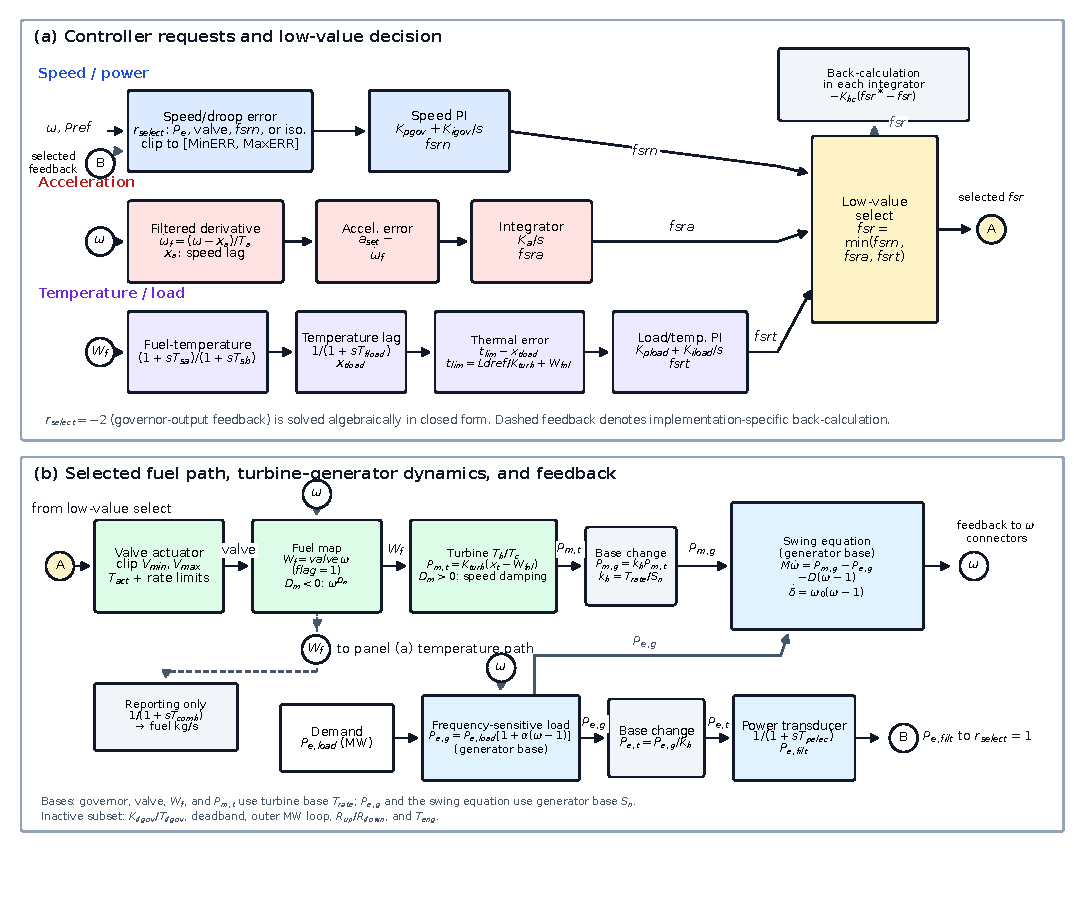
\includegraphics[width=\textwidth]{ggov1_implementation_block_diagram.pdf}
  \caption{Implementation-oriented GGOV1 block diagram.  Panel (a) shows the
  three controller requests and low-value decision.  Panel (b) shows the
  selected valve/fuel/turbine path, generator dynamics, electrical-load path,
  and named feedback connectors.  Solid arrows are forward decision flow;
  dashed arrows are feedback or reporting paths.}
  \label{fig:block}
\end{figure}

\clearpage
%=====================================================================
\section{How the six test cases were constructed}
%=====================================================================

All scenarios are generated by
\path{tools/vv/plot_ggov1_explainer.py} using the implementation in
\path{gas_plant/dynamics/ggov1.py}.  Unless a case says otherwise, the
parameters come from \texttt{GGOV1Params.lm2500\_overrides()}: IEEE PES-TR1
Appendix-C typical values with a faster $T_{act}=\SI{0.15}{s}$ actuator and
$R=0.04$ droop.  Table~\ref{tab:cases} summarizes the disturbances.

\begin{table}[htbp]
\centering
\caption{Summary of the six explanatory cases.}
\label{tab:cases}
\small
\begin{tabular}{@{}p{0.07\textwidth}p{0.28\textwidth}p{0.28\textwidth}p{0.28\textwidth}@{}}
\toprule
Case & Scenario & Main behavior & Principal question \\
\midrule
1 & Load step \SI{11.5}{MW} $\rightarrow$ \SI{14}{MW} & Power mismatch, frequency nadir, recovery & Why does frequency fall after load increases? \\
2 & Same \SI{2.5}{MW} load increase & \fsrn/\fsra/\fsrt arbitration and valve lag & Which controller actually determines fuel? \\
3 & Same load step in droop and isochronous modes & Different steady-state frequency objectives & Why does droop retain a frequency offset? \\
4 & Overload \SI{15}{MW} $\rightarrow$ \SI{25}{MW} & Transient headroom followed by thermal-limit takeover & Why is short-term power not sustained capability? \\
5 & Load rejection \SI{15}{MW} $\rightarrow$ \SI{8}{MW} & Overspeed tendency and acceleration protection & How does GGOV1 cut fuel after load disappears? \\
6 & Hannett Table-3-style benchmark & Response-speed and speed-excursion metrics & Is the modeled response in the neighborhood of published gas-turbine results? \\
\bottomrule
\end{tabular}
\end{table}

\begin{cautionbox}[Educational tests versus complete validation]
Cases 1--5 are controlled numerical demonstrations.  They verify that the
implemented loops interact in a physically understandable way, but they are
not measurements from an LM2500 and do not establish model-parameter accuracy.
Case 6 supplies literature context, but even that comparison is limited by
unpublished plant parameters and differences between machines.  These figures
should support explanation and software verification, not a claim of OEM-grade
LM2500 certification.
\end{cautionbox}

%=====================================================================
\section{Case 1: normal load increase and frequency recovery}
%=====================================================================

\subsection{Question and setup}
At $t=0$ on the figure's relative time axis, electrical demand changes from
\SI{11.5}{MW} to \SI{14}{MW}.  The physical step is applied at
$t=\SI{5}{s}$ in the simulation; subtracting five seconds simply makes the
plot easier to read.  The plotted window emphasizes the first ten seconds,
where the important governor dynamics occur.

\subsection{Expected sequence}
\begin{enumerate}
  \item Electrical demand changes almost instantaneously.
  \item Mechanical turbine power initially remains near its old value because
        the controller, actuator, fuel flow, and turbine all require time.
  \item The negative power imbalance causes frequency to fall according to
        Equation~\eqref{eq:swing}.
  \item The speed/power governor raises its fuel request.  The valve opens at a
        finite rate and turbine mechanical power rises.
  \item As $\Pm$ approaches $\Pe$, the frequency decline stops at the
        \emph{nadir}; frequency then recovers toward its controlled value.
\end{enumerate}

\begin{figure}[htbp]
  \centering
  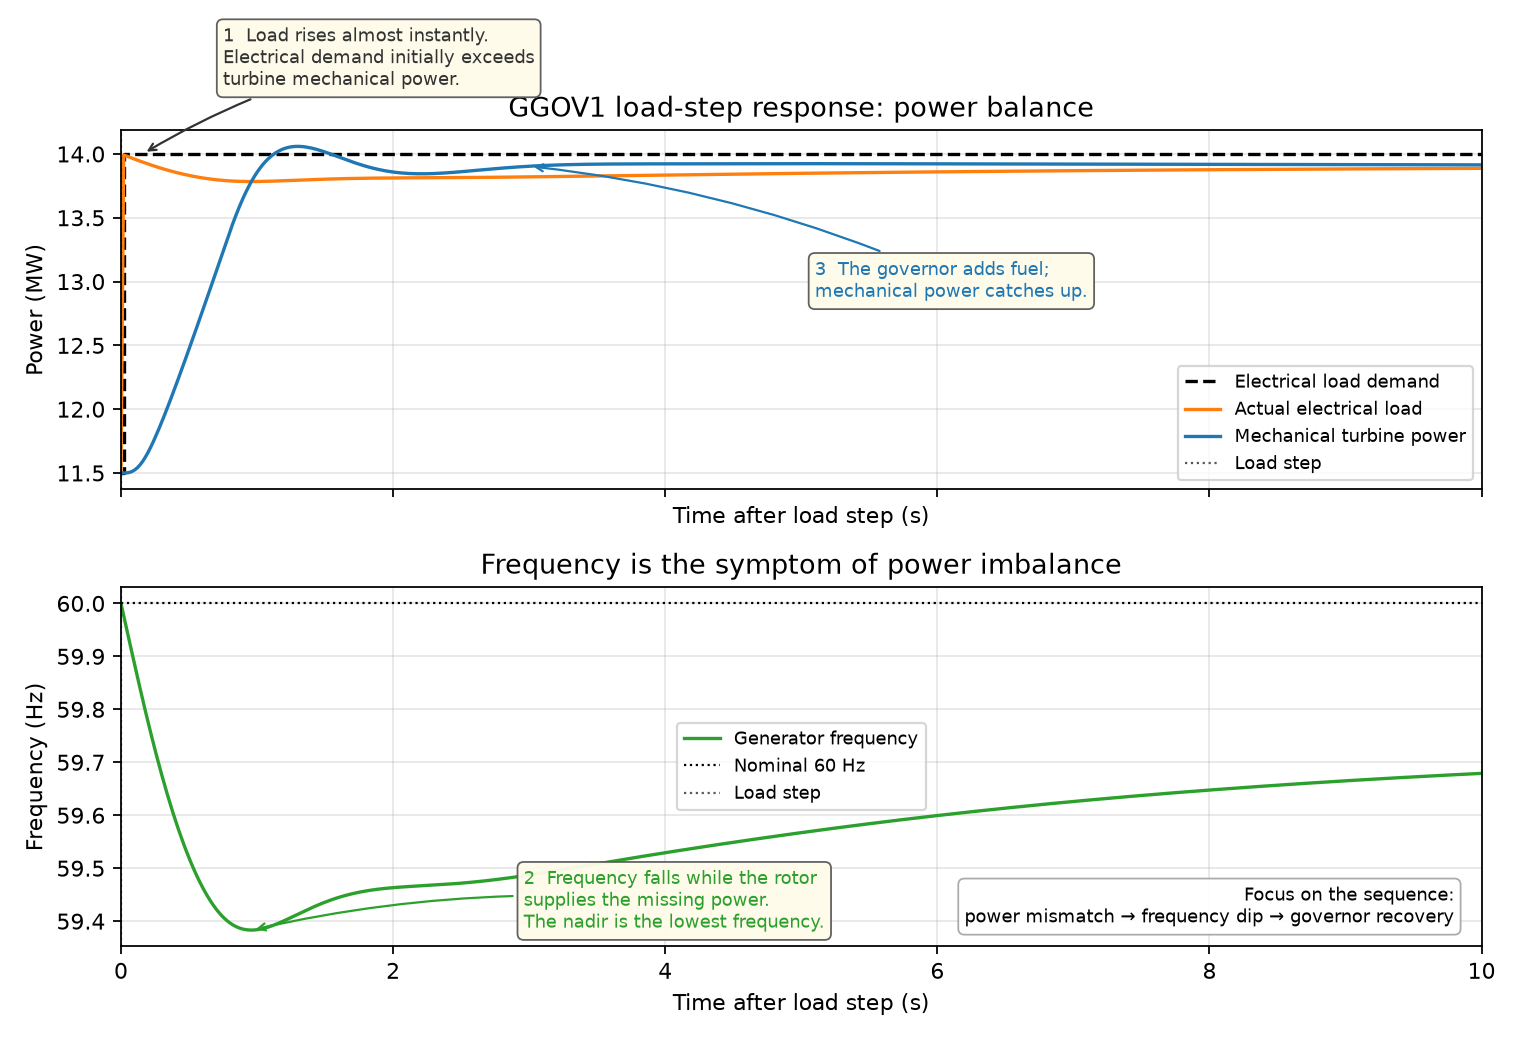
\includegraphics[width=0.94\textwidth]{ggov1_01_load_step_story.png}
  \caption{Case 1: cause-and-effect story for a normal load increase.  The
  upper panel shows demand, actual frequency-sensitive electrical load, and
  turbine mechanical power.  The lower panel shows the resulting generator
  frequency.  Numbered annotations give the intended reading order.}
  \label{fig:case1}
\end{figure}

\begin{focusbox}[Case 1]
Do not read the frequency dip as a separate phenomenon.  Compare the upper and
lower panels at the same time.  Frequency falls precisely while mechanical
power is below electrical power.  The nadir occurs near the time when that
imbalance is being removed.  Also distinguish the dashed demand trace from the
orange actual electrical-load trace: the latter includes the model's
frequency-sensitive load damping.
\end{focusbox}

\subsection{What this case tests}
This case checks the sign and ordering of the coupled dynamics: increased load
must produce a frequency decline, governor fuel must increase, mechanical
power must follow with a delay, and the frequency response must stabilize.  A
wrong sign in the swing equation or governor feedback would make frequency
move in the wrong direction or diverge.

%=====================================================================
\section{Case 2: low-value selection and valve lag}
%=====================================================================

\subsection{Why three request signals are shown}
Each GGOV1 branch continuously computes the fuel stroke it would choose:
\begin{itemize}
  \item \fsrn: normal speed/power request, plotted blue;
  \item \fsra: acceleration-protection request, plotted red;
  \item \fsrt: temperature/load-protection request, plotted purple.
\end{itemize}
The thick black line is the selected minimum from Equation~\eqref{eq:lvg}.
The green line is the physical valve stroke after Equation~\eqref{eq:valve}.
These are not interchangeable: $\fsr$ is a command, while $v$ is a state of a
physical actuator.

\begin{figure}[htbp]
  \centering
  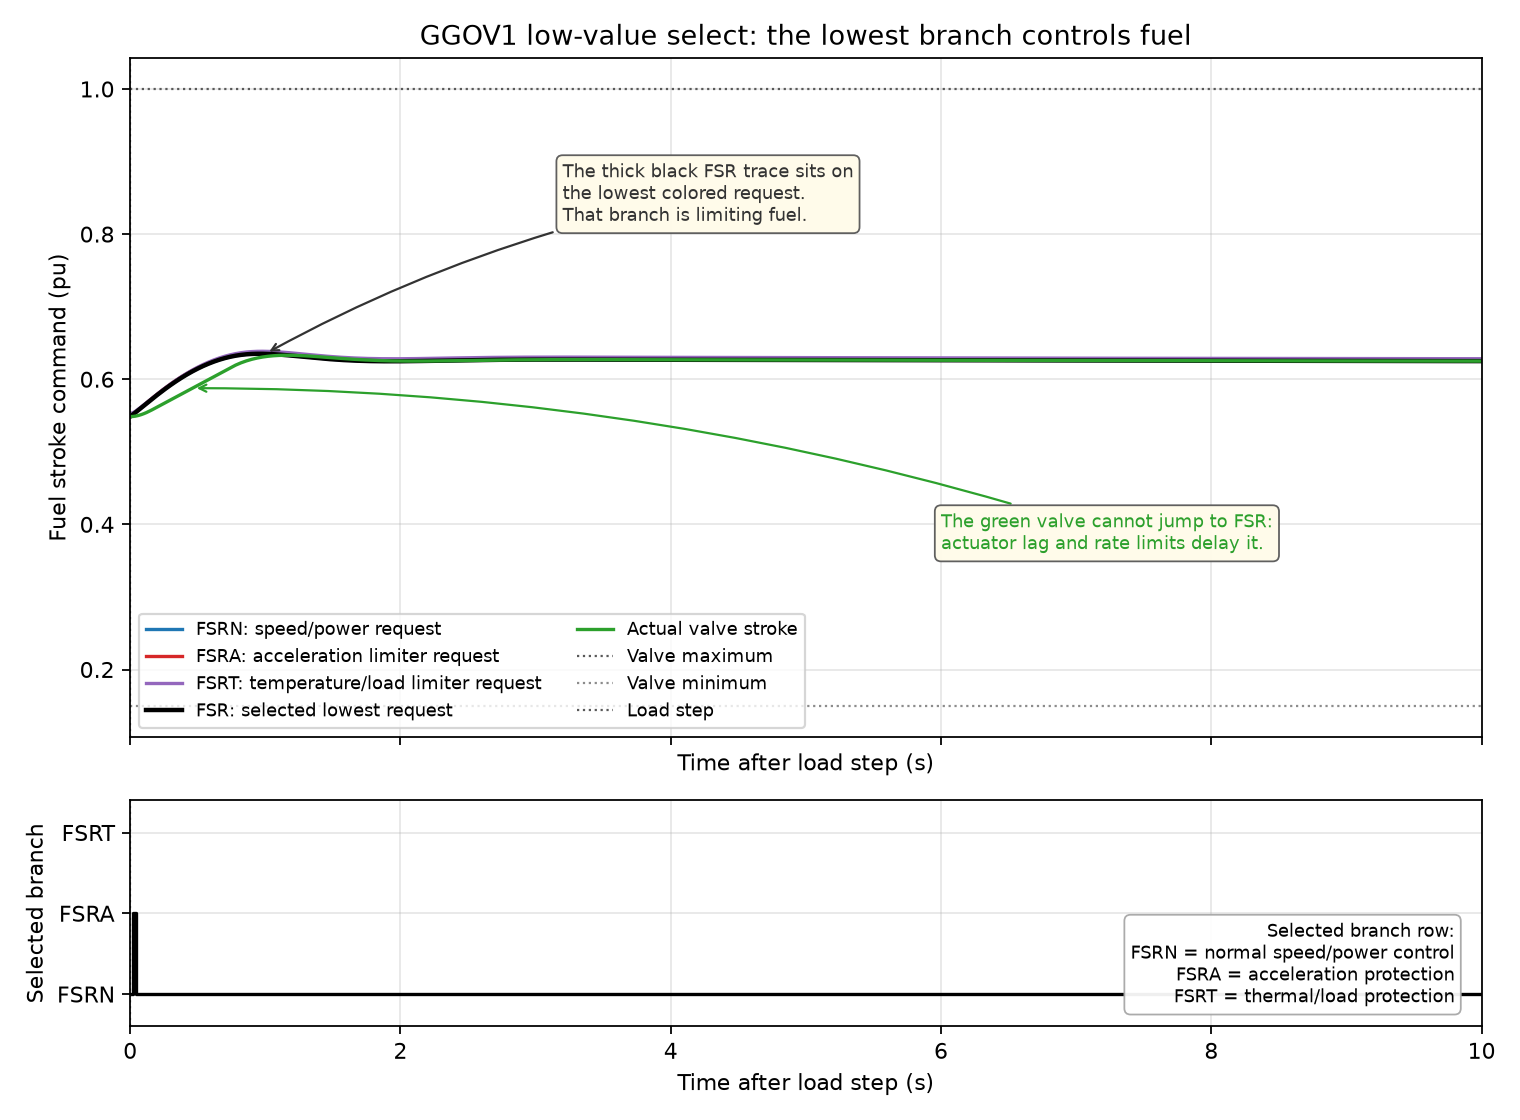
\includegraphics[width=0.94\textwidth]{ggov1_02_controller_arbitration.png}
  \caption{Case 2: GGOV1 controller arbitration during the same normal load
  increase as Case 1.  The bottom panel converts the minimum calculation into
  a categorical view of the active branch.}
  \label{fig:case2}
\end{figure}

\begin{focusbox}[Case 2]
First find the thick black $\fsr$ line and identify which colored request lies
under it.  Then look at the categorical bottom panel for confirmation.  Finally
compare black $\fsr$ with green valve stroke.  Their separation is the visible
consequence of actuator lag and valve-rate limits; it is not a controller
selection error.
\end{focusbox}

\subsection{Anti-windup behavior}
When one branch is selected, the other controller integrators could otherwise
continue accumulating error, or ``wind up.''  The implementation applies
back-calculation:
\begin{align}
  \dot x_{igov} &= K_{igov}e_{speed}
    -K_{bc,speed}(\fsrn-\fsr),\\
  \dot x_a &= K_ae_{accel}
    -K_{bc,accel}(\fsra-\fsr),\\
  \dot x_{iload} &= K_{iload}e_{temp}
    -K_{bc,temp}(\fsrt-\fsr).
\end{align}
The tracking terms pull unselected branches toward the winning command so a
later handoff is smoother.

\subsection{What this case tests}
The case checks that the numerical low-value gate agrees with the plotted
active-branch category, that normal operation is not unintentionally dominated
by a protective branch, and that valve motion respects its own dynamics rather
than jumping directly to the controller request.

%=====================================================================
\section{Case 3: droop versus isochronous control}
%=====================================================================

\subsection{Two different control objectives}
The disturbance is again \SI{11.5}{MW} to \SI{14}{MW}, but the simulation is
run twice.

\paragraph{Droop mode ($rselect=1$).}
Electrical power passes through the $T_{pelec}$ transducer and participates in
the speed-governor error.  In simplified form,
\begin{equation}
  e_{speed}=(1-\omega)+R(P_{ref}-P_{e,filt}).
  \label{eq:droop}
\end{equation}
Droop intentionally permits a steady frequency offset as load changes.  This
behavior allows multiple generators to share a load change without every
controller trying to force the system independently to exactly \SI{60}{Hz}.

\paragraph{Isochronous mode ($rselect=0$).}
Power feedback is removed:
\begin{equation}
  e_{speed}=1-\omega.
  \label{eq:iso}
\end{equation}
The integral controller continues adjusting fuel until steady frequency
returns to nominal.  Isochronous control is natural for one designated master
unit in an island, but several independent isochronous governors can fight one
another unless coordinated.

\begin{figure}[htbp]
  \centering
  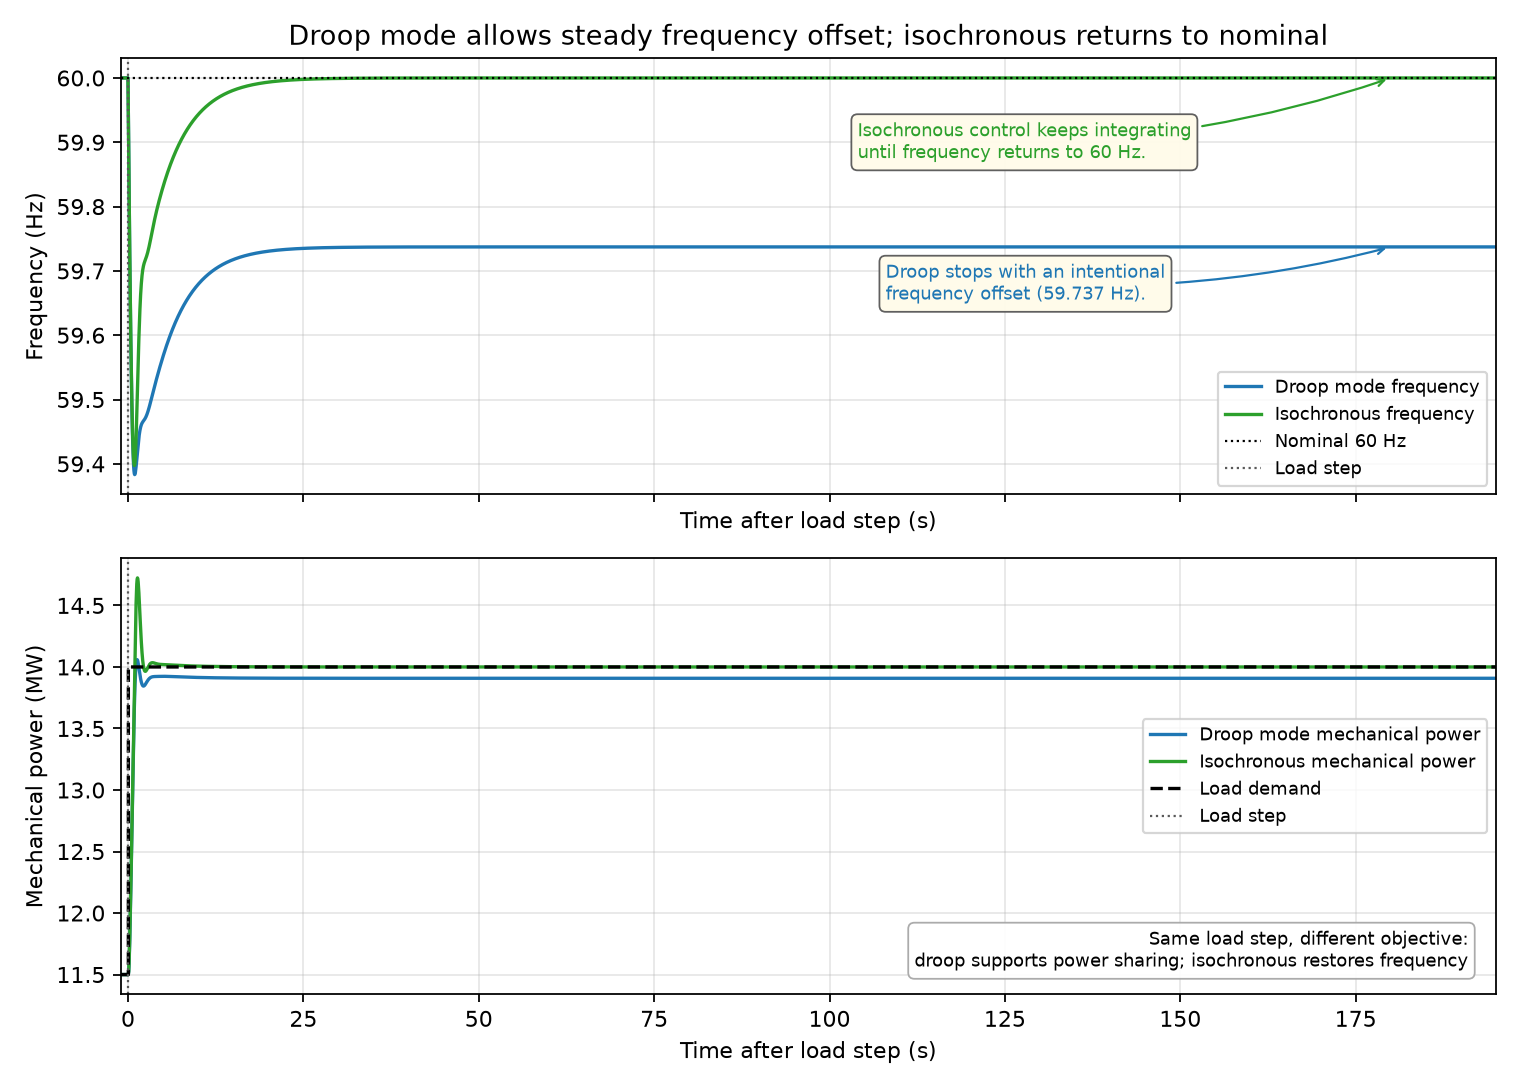
\includegraphics[width=0.94\textwidth]{ggov1_03_droop_vs_isochronous.png}
  \caption{Case 3: frequency and mechanical-power response for droop and
  isochronous control.  Both cases stabilize, but their steady-state objectives
  differ.}
  \label{fig:case3}
\end{figure}

\begin{focusbox}[Case 3]
Focus on the final values, not only the initial dip.  The blue droop trace
settles with a deliberate frequency error; the green isochronous trace returns
toward \SI{60}{Hz}.  This does not make isochronous control universally
``better.''  Droop provides decentralized power sharing, while isochronous
control provides exact frequency restoration for a suitable master unit.
\end{focusbox}

\subsection{What this case tests}
This test exercises two code paths selected by \texttt{rselect}.  It confirms
that electrical-power droop feedback is active for $rselect=1$ and omitted for
$rselect=0$, and that the long-term responses reflect those different control
laws.

%=====================================================================
\section{Case 4: overload request and thermal-limiter takeover}
%=====================================================================

\subsection{Setup and two different power ceilings}
The requested load increases from \SI{15}{MW} to \SI{25}{MW}.  This request is
above the model's continuous thermal reference:
\begin{equation}
  P_{thermal,max}=Ldref\,T_{rate}=1.0\times\SI{22}{MW}=\SI{22}{MW}.
\end{equation}
The valve can temporarily produce a higher idealized mechanical ceiling:
\begin{equation}
  P_{transient,max}=K_{turb}(V_{max}-W_{fnl})T_{rate}
  =1.5(1.0-0.2)\times\SI{22}{MW}=\SI{26.4}{MW}.
\end{equation}
The difference between \SI{26.4}{MW} transient capability and \SI{22}{MW}
continuous capability is central to the case.

\subsection{Temperature-path logic}
The implementation uses fuel flow as a temperature/load proxy.  It passes
through a lead--lag and a lag, then compares with the fuel level corresponding
to the thermal reference:
\begin{equation}
  t_{lim}=\frac{Ldref}{K_{turb}}+W_{fnl},\qquad
  e_{temp}=t_{lim}-x_{tload},
\end{equation}
\begin{equation}
  \fsrt=K_{pload}e_{temp}+x_{iload}.
\end{equation}
As the filtered fuel proxy rises, \fsrt becomes more restrictive.  Once it is
below \fsrn, the low-value gate selects it and sustained fuel is reduced.

\begin{figure}[htbp]
  \centering
  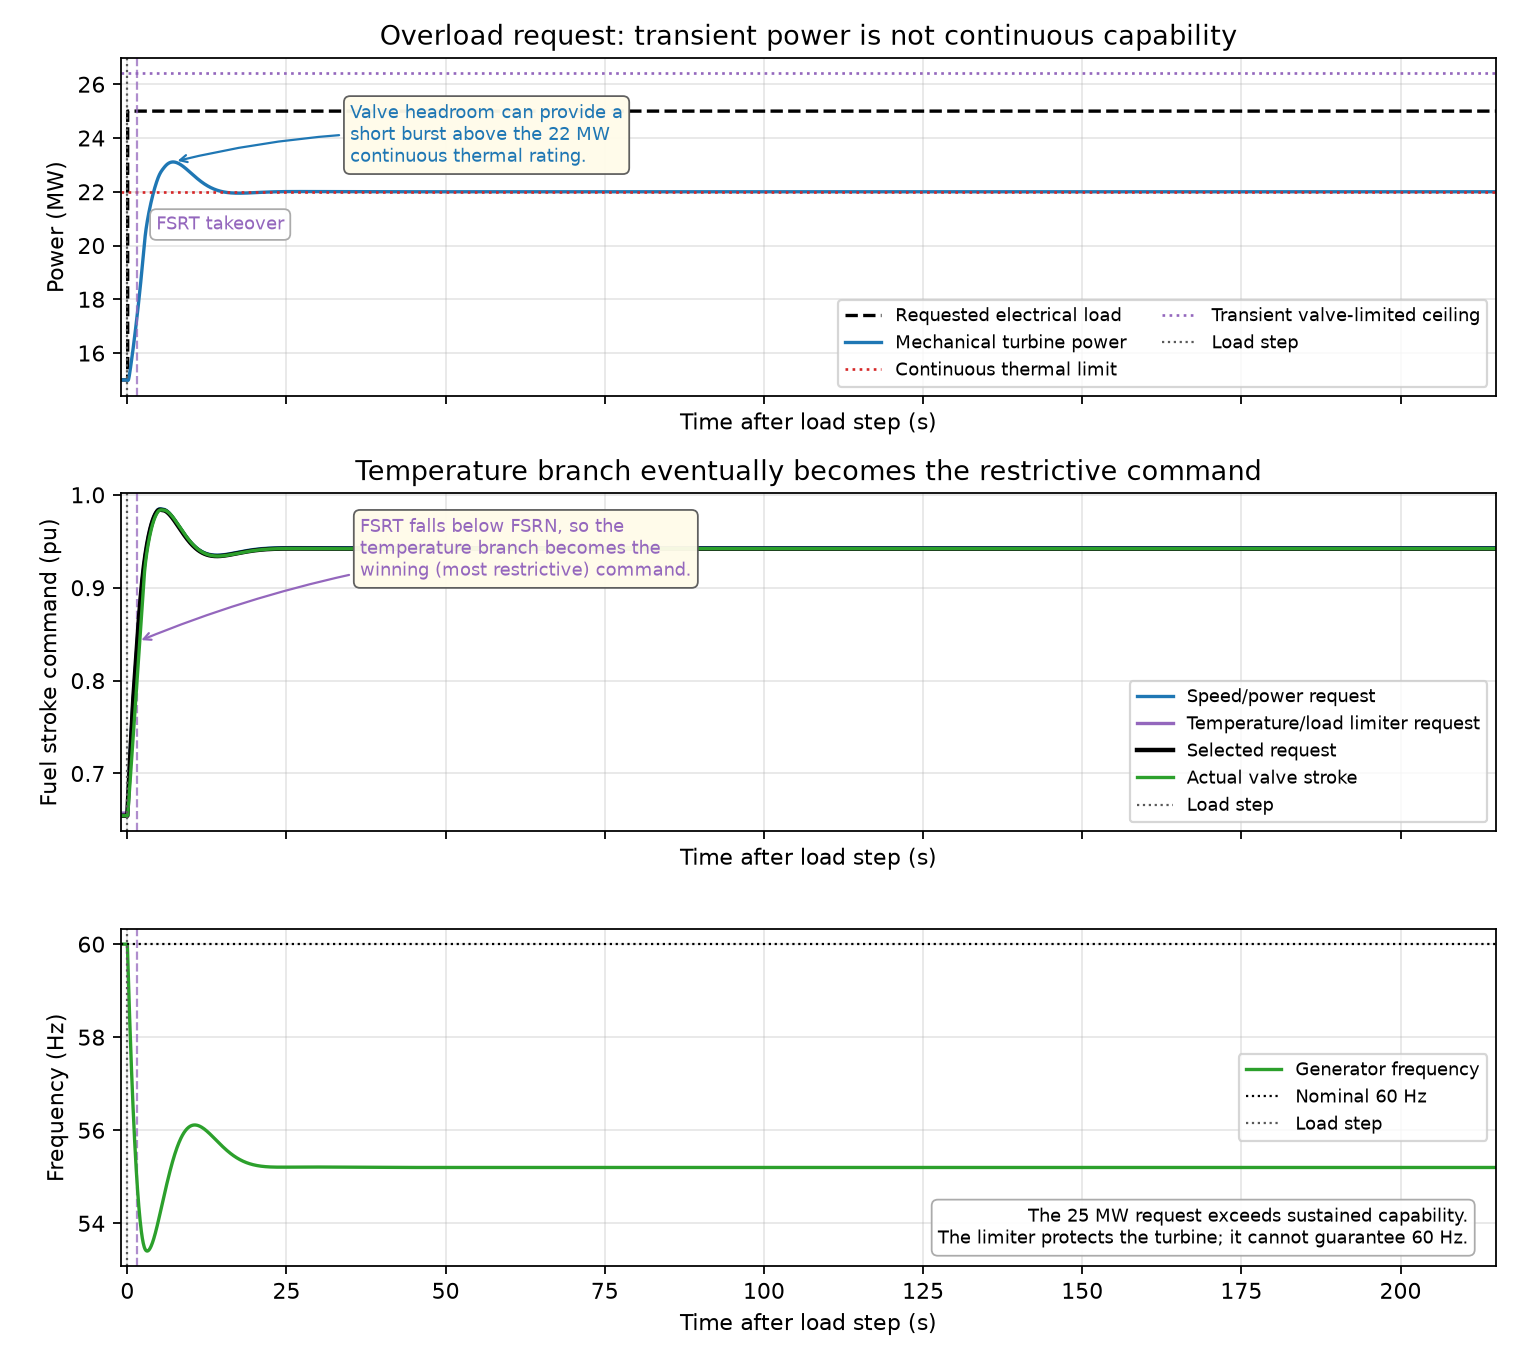
\includegraphics[width=0.94\textwidth]{ggov1_04_thermal_limiter_takeover.png}
  \caption{Case 4: an overload request produces transient mechanical-power
  headroom, followed by takeover of the temperature/load branch.  The purple
  dashed vertical line identifies sustained \fsrt selection.}
  \label{fig:case4}
\end{figure}

\begin{focusbox}[Case 4]
The \SI{25}{MW} dashed load request is not a promise that the turbine can
supply \SI{25}{MW} indefinitely.  Read the panels together: temporary valve
headroom raises mechanical power, then purple \fsrt falls below blue \fsrn and
becomes the selected request.  Frequency remains low because protecting the
turbine and satisfying an infeasible load request are conflicting objectives.
\end{focusbox}

\begin{cautionbox}[Temperature is represented by a proxy]
This repository does not solve combustor metal temperature, exhaust-temperature
thermocouple dynamics, blade cooling, or OEM thermal-control logic.  The GGOV1
load-limiter path is a standard reduced-order control representation driven by
fuel flow.  The case verifies the implemented limiter architecture; it does not
predict component temperature or prove an LM2500 overload duration.
\end{cautionbox}

%=====================================================================
\section{Case 5: load rejection and acceleration protection}
%=====================================================================

\subsection{Setup}
Electrical load falls from \SI{15}{MW} to \SI{8}{MW}.  Immediately after the
rejection, fuel and mechanical torque remain near their pre-event values, but
electrical braking torque has decreased.  Therefore $\Pm>\Pe$, the right side
of Equation~\eqref{eq:swing} is positive, and the rotor accelerates.

\subsection{Filtered acceleration and protective request}
A raw numerical derivative of speed is noisy.  GGOV1 uses a filtered
derivative based on a first-order speed-lag state:
\begin{equation}
  \dot x_{accel,lag}=\frac{\omega-x_{accel,lag}}{T_a},\qquad
  a_f=\frac{\omega-x_{accel,lag}}{T_a}.
\end{equation}
The acceleration error is
\begin{equation}
  e_{accel}=a_{set}-a_f,
\end{equation}
and the acceleration branch is a pure integrator request:
\begin{equation}
  \begin{aligned}
    \fsra &= x_a,\\
    \dot x_a &= K_ae_{accel}\\
             &\quad{}-K_{bc,accel}(\fsra-\fsr).
  \end{aligned}
\end{equation}
When acceleration exceeds its setpoint, $e_{accel}<0$.  This negative error
drives \fsra downward.

If \fsra becomes the lowest request, the low-value gate commands a rapid fuel
reduction.

\begin{figure}[htbp]
  \centering
  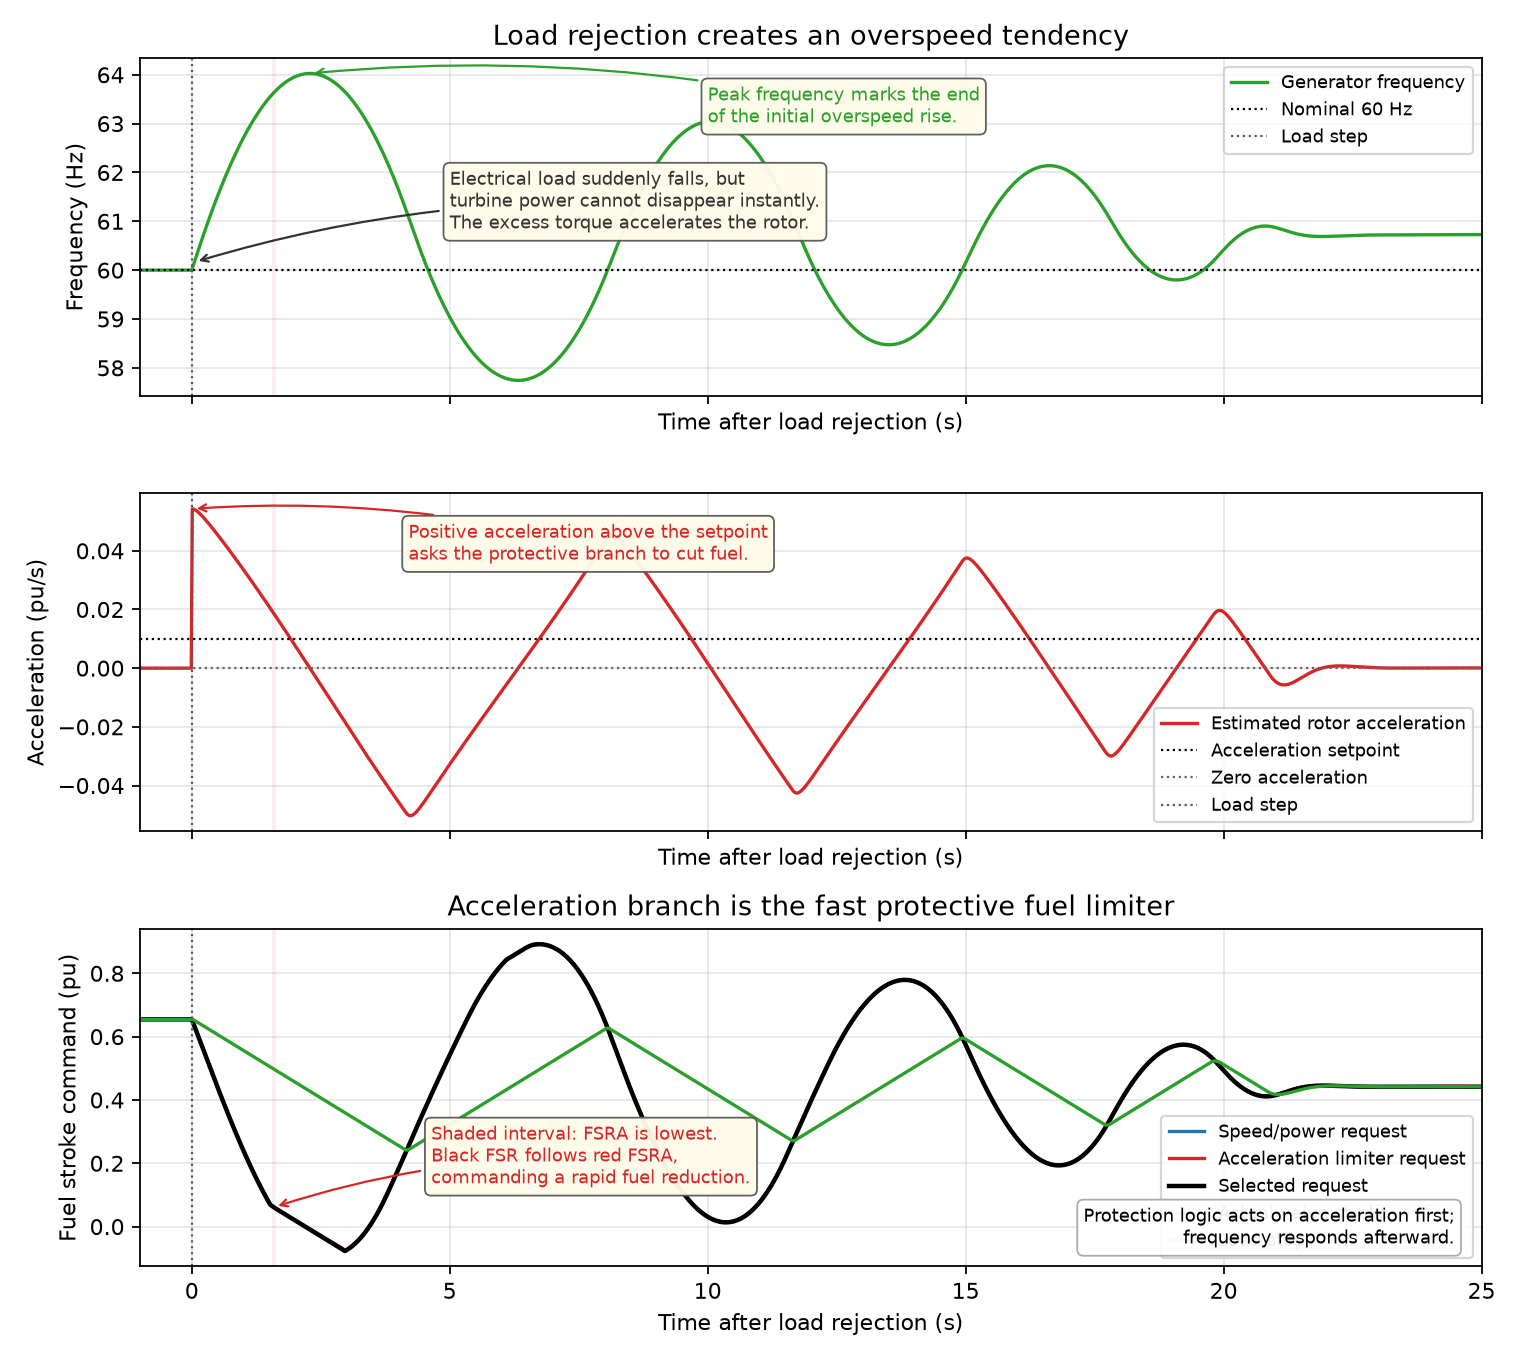
\includegraphics[width=0.94\textwidth]{ggov1_05_acceleration_limiter.png}
  \caption{Case 5: frequency, estimated acceleration, and controller requests
  after a load rejection.  Light red shading marks the interval during which
  the acceleration branch is selected.}
  \label{fig:case5}
\end{figure}

\begin{focusbox}[Case 5]
Follow the panels from the disturbance downward.  Load rejection first creates
excess mechanical torque.  Positive acceleration appears before frequency has
reached its maximum.  During the shaded interval, red \fsra is the lowest
request and black \fsr follows it, cutting fuel.  The green valve follows more
slowly because physical actuator constraints still apply.
\end{focusbox}

\subsection{What this case tests}
The case checks disturbance sign, filtered-derivative behavior, acceleration
setpoint comparison, low-value selection of \fsra, and subsequent reduction of
fuel.  It is a structural protection test; it is not a certification of
overspeed-trip settings or shaft-stress limits.

%=====================================================================
\section{Case 6: published validation context}
%=====================================================================

\subsection{Why a literature comparison is needed}
Cases 1--5 can show that software behaves coherently, but coherent behavior can
still come from incorrectly tuned equations.  Case 6 compares response metrics
with Hannett and Khan's published gas-turbine model-validation study.  The
protocol represented here starts at 50\% of generator MVA rating and applies a
10\% rating load increase, with 3\% droop.  For the repository's
$S_n=\SI{23}{MVA}$ generator, this corresponds to
\begin{equation}
  P_0=0.5S_n=\SI{11.5}{MW},\qquad
  P_1=0.6S_n=\SI{13.8}{MW}.
\end{equation}

\subsection{The two benchmark metrics}
\paragraph{Time to 0.6 pu mechanical power.}
This is the time after the disturbance at which mechanical power first reaches
$0.6\pu$ on generator base.  A shorter time indicates a faster turbine and
governor response.

\paragraph{Maximum rotor-speed excursion.}
For a load increase the excursion is negative because speed falls.  A value
closer to zero means a smaller frequency dip.  At a \SI{60}{Hz} base, for
example, $-0.004\pu$ corresponds to approximately
$60(-0.004)=\SI{-0.24}{Hz}$.

The two published anchors plotted are
\begin{center}
\begin{tabular}{@{}lcc@{}}
\toprule
Published anchor & Time to $0.6\pu$ & Minimum speed excursion \\
\midrule
Hannett typical model & \SI{1.140}{s} & $-0.0039\pu$ \\
Hannett field-derived model & \SI{2.320}{s} & $-0.0076\pu$ \\
\bottomrule
\end{tabular}
\end{center}
The repository then runs GGOV1 with PES-TR1 typical values, GGOV1 with LM2500
overrides, and a Rowen typical-gas model under the same simplified protocol.

\begin{figure}[htbp]
  \centering
  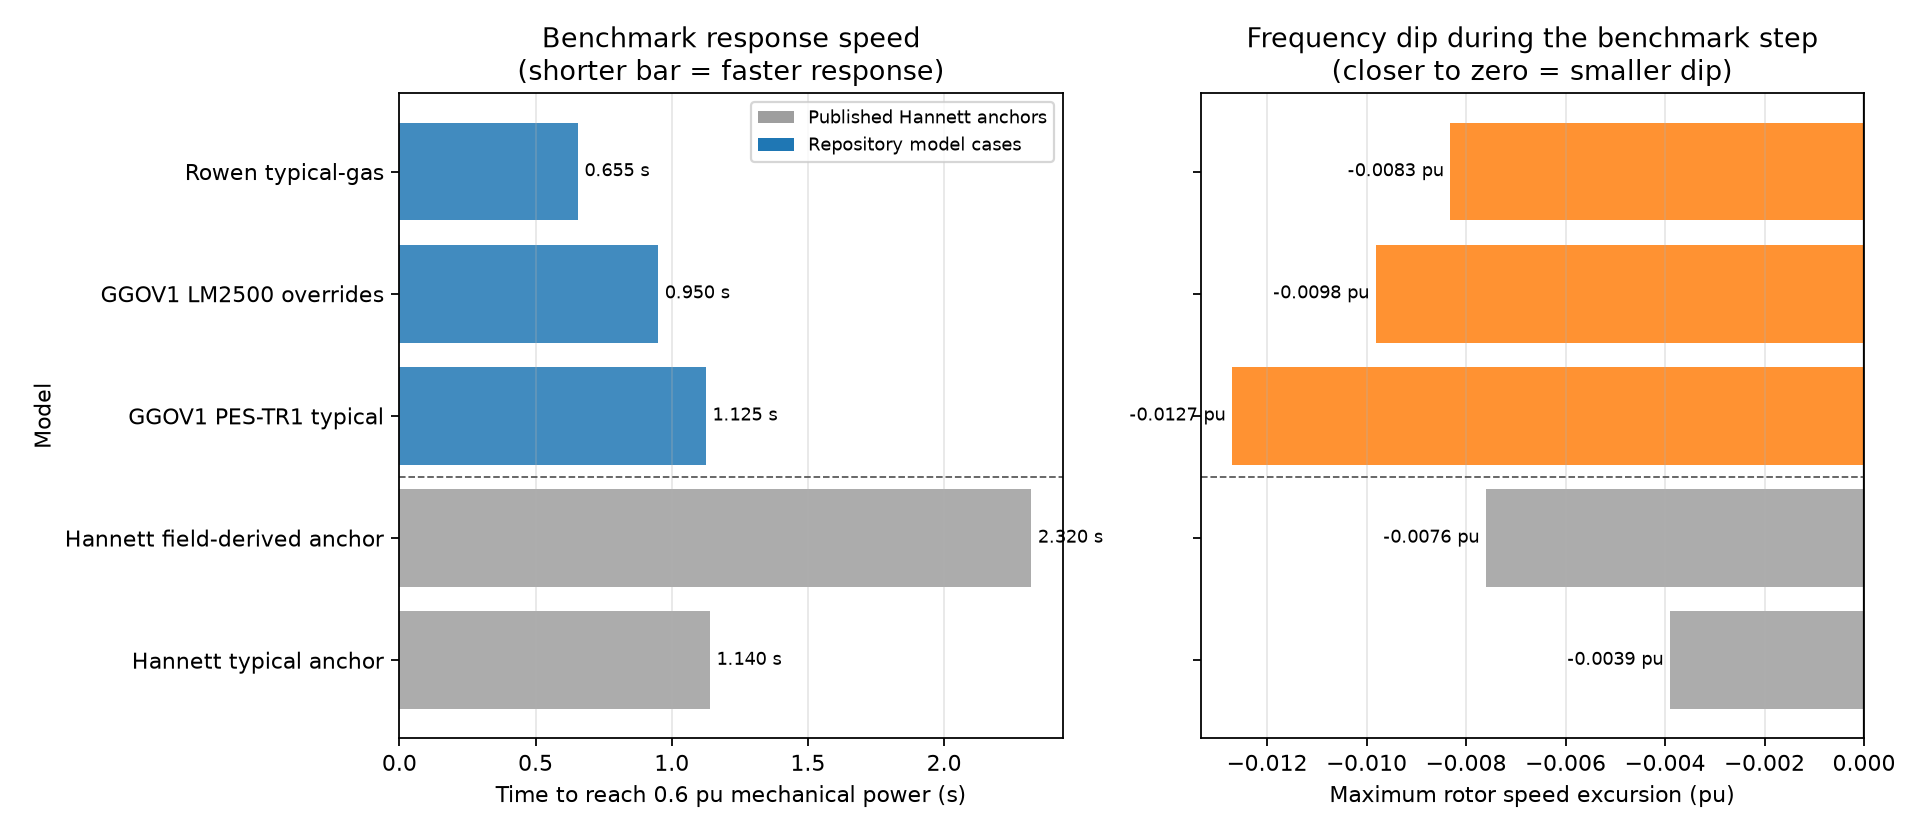
\includegraphics[width=\textwidth]{ggov1_06_validation_context.png}
  \caption{Case 6: published Hannett anchors (gray) and repository model cases
  (colored).  The left panel compares response speed; the right compares the
  maximum speed/frequency dip.  The dashed horizontal line separates published
  anchors from repository simulations.}
  \label{fig:case6}
\end{figure}

\begin{focusbox}[Case 6]
Do not select a model by matching only one bar.  A model could reach mechanical
power quickly by being unrealistically aggressive and simultaneously produce a
wrong speed excursion.  Credibility requires reasonable agreement in response
time, speed excursion, waveform shape, and the parameter assumptions behind
the comparison.
\end{focusbox}

\begin{cautionbox}[What the bars do not prove]
The Hannett anchors are from other gas-turbine units and model parameter sets,
not a controlled test on this repository's specific LM2500.  Similar bars show
that the response is in a plausible published neighborhood.  They do not
uniquely identify actuator constants, inertia, thermal limits, or an OEM
controller implementation.  Field data from the actual generator package
would be required for high-confidence LM2500 calibration.
\end{cautionbox}

%=====================================================================
\section{Fleet study: what changes when 2, 3, or 4 units share the load?}
\label{sec:fleet}
%=====================================================================

The six preceding cases explain one governor in controlled disturbances.
The script \path{tools/vv/fleet_study.py} asks a different, practical
question: how many identical LM2500-class units are needed to follow a rapidly
changing data-center load, and what torsional fatigue does one shaft
experience while doing so?  This section explains the code from input data to
reported results.

\begin{novicebox}[What ``fleet'' means in this study]
The script does not simulate several independently controlled generators and
a detailed electrical network.  It replaces $N$ identical, equally sharing
units on one common bus with one \emph{aggregated equivalent machine}.  Its
power and MVA ratings are $N$ times those of one unit, while its per-unit
control parameters are unchanged.  This is a standard screening
approximation, but it cannot reveal unequal load sharing, circulating power,
unit-to-unit oscillation, breaker behavior, or network voltage effects.

This dynamic aggregation is also separate from the steady-state
\path{gas_plant/fleet.py} dispatch helper.  The fleet study directly calls the
GGOV1, multishaft, and torsional dynamic models.
\end{novicebox}

\subsection{Step 1: construct the two-hour electrical-load trace}

The function \texttt{build\_trace()} reads
\path{data/nvidia_smi_first_1gb.parquet}.  Each row is a measured GPU power
sample.  The code performs the following operations:
\begin{enumerate}
  \item Sort all records by time and find the two-hour interval containing
        the densest measurement activity.
  \item Create a \,\SI{0.1}{s} time grid.  For each node and GPU, retain the
        last observation in a slot and hold that value until the next sample.
        This is a zero-order hold, not an interpolation that invents smooth
        ramps between measurements.
  \item Sum the reconstructed GPU powers into a raw IT-load signal $B(t)$.
  \item Apply a power-usage effectiveness value of $1.25$.  The added
        non-IT load is represented as $0.25$ times the mean IT load.
  \item Scale the resulting waveform so its maximum is \SI{18}{MW}.
\end{enumerate}
For this run, the constructed facility load spans \SI{5.2}{MW} to
\SI{18.0}{MW}.  Its largest downward and upward single-sample changes are
$-\SI{10.5}{MW}$ and $+\SI{9.6}{MW}$, respectively.

\begin{cautionbox}[The trace is a conservative constructed scenario]
The scaling treats the sampled GPU activity as if enough similar devices were
perfectly synchronized to create an \SI{18}{MW} peak.  It is useful as a
stress test, but it is not a measured \SI{18}{MW} facility feeder trace.
Real workload diversity, power-supply controls, UPS equipment, batteries, and
network constraints may substantially change the waveform seen by a turbine.
\end{cautionbox}

\subsection{Step 2: represent $N$ turbines as one dynamic equivalent}

The function \texttt{run\_fleet()} creates a GGOV1 parameter set with
\begin{equation}
  S_N=N(\SI{23}{MVA}), \qquad T_{rate}=N(\SI{22}{MW}),
  \label{eq:fleet-bases}
\end{equation}
for $N=2$, $3$, and $4$.  Thus the fleets have generator bases of
\SI{46}{MVA}, \SI{69}{MVA}, and \SI{92}{MVA}, and turbine ratings of
\SI{44}{MW}, \SI{66}{MW}, and \SI{88}{MW}.  The turbine-to-generator base
ratio remains
\begin{equation}
  k_b=\frac{T_{rate}}{S_N}=\frac{22}{23},
\end{equation}
independent of fleet size.

The aggregated machine is passed to \texttt{simulate\_multishaft()}.  This
Tier-C model has 13 dynamic states: the GGOV1 controller and turbine states,
the power-turbine/generator rotor angle and speed, and an HP gas-generator
speed.  Its power-turbine/generator speed follows the familiar balance
\begin{equation}
  2H_{PT}\frac{d\omega_{PT}}{dt}
  =P_{couple}k_b-P_e-D_{PT}(\omega_{PT}-1).
  \label{eq:fleet-swing}
\end{equation}
The present model uses $H_{PT}=\SI{2.5}{s}$ and $D_{PT}=0$; frequency-sensitive
load is represented in $P_e$ instead of being counted a second time as
machine damping.  Because the same MW disturbance is divided by a larger
base as $N$ grows, it becomes a smaller per-unit disturbance.  The aggregate
stored rotor energy and total valve-moving capability also increase with
$N$.  Therefore a larger fleet should exhibit a smaller frequency excursion.

The HP rotor is coupled to the power turbine by the reduced-order gas-path law
\begin{equation}
  P_{couple}=K_{couple}(\omega_{HP}-\omega_{HP,idle}).
\end{equation}
This is a linear placeholder, not a detailed compressor and turbine map.

\subsection{Step 3: select a demanding 15-minute screening interval}

The script locates the largest absolute one-sample load change and extracts
\SI{900}{s} around it.  Each $N$ value is first simulated on this same segment
with a \SI{0.02}{s} output interval.  The \texttt{report()} function computes:
\begin{itemize}
  \item minimum and maximum electrical frequency;
  \item total sampled time below \SI{57.8}{Hz}, used here as an
        instantaneous-trip screening threshold; and
  \item time outside the \SIrange{59.4}{60.6}{Hz} continuous operating band.
\end{itemize}
These are screening criteria rather than a complete relay model.  In
particular, ``time below \SI{57.8}{Hz}'' is the sum of samples below the
threshold; an actual protection system would normally trip at the first
qualifying event and the later simulated trajectory would never occur.

\subsection{Step 4: calculate per-shaft torsional fatigue only if the unit survives}

For a surviving trajectory, \texttt{per\_shaft\_fatigue()} makes a shallow
copy of the fleet result and divides mechanical and electrical power by $N$:
\begin{equation}
  P_{m,unit}=\frac{P_{m,fleet}}{N},\qquad
  P_{e,unit}=\frac{P_{e,fleet}}{N}.
  \label{eq:per-shaft-power}
\end{equation}
It then drives one \SI{23}{MVA} two-mass shaft model.  The power-turbine rotor
and generator rotor are connected by a torsional spring and damper:
\begin{align}
  2H_{PT,o}\dot\omega_{PT,o} &= \tau_{in}-\tau_{shaft},\\
  2H_{gen}\dot\omega_{gen} &= \tau_{shaft}-\tau_e,\\
  \tau_{shaft} &= k\theta+c(\omega_{PT,o}-\omega_{gen}).
  \label{eq:torsional-fleet}
\end{align}
The assumed torsional mode is \SI{22}{Hz}.  The model samples shaft torque at
\SI{500}{Hz}, which is fast enough to resolve that mode.

A centered \SI{5}{s} rolling median separates torque into a slow trend and a
high-frequency residual.  Rainflow counting converts each history into
equivalent load cycles.  Miner's rule sums the fractional damage,
\begin{equation}
  D=\sum_i\frac{n_i}{N_{f,i}},
\end{equation}
where $n_i$ is the counted number of cycles and $N_{f,i}$ is the predicted
number of cycles to failure at that amplitude.  The Basquin relation used to
obtain $N_f$ has the form
\begin{equation}
  N_f=N_{ref}\left(\frac{S_{a,ref}}{S_{a,eq}}\right)^m.
  \label{eq:basquin}
\end{equation}
The high-cycle-fatigue (HCF) residual uses $m=9$; the slow
low-cycle-fatigue (LCF) trend uses $m=4$.  A Goodman correction increases the
equivalent alternating stress when nonzero mean torque is present.

If every unit saw the same cycles and only the torque amplitude changed as
$1/N$, Equation~\ref{eq:basquin} would imply
\begin{equation}
  D_{unit}\propto N^{-m},\qquad
  \frac{D_3}{D_4}\approx\left(\frac{4}{3}\right)^m.
  \label{eq:fleet-basquin-scaling}
\end{equation}
The actual simulations need not obey this exactly because changing $N$ also
changes the governor and rotor trajectory, and therefore changes the cycles
being counted.

\subsection{Results for $N=2$, $N=3$, and $N=4$}

Table~\ref{tab:fleet-segment} reports the newly executed 15-minute screening
cases.  Fatigue is deliberately omitted for $N=2$: it spends
\SI{235.1}{s} below the trip threshold, so the model's later shaft history
describes a generator that should already have disconnected.

\begin{table}[htbp]
\centering
\caption{Worst-segment fleet screening results from
\texttt{pixi run vv-fleet}.}
\label{tab:fleet-segment}
\small
\begin{tabular}{@{}crrrr@{}}
\toprule
$N$ & Frequency range (Hz) & Below \SI{57.8}{Hz} (s) & Out of band (s) & Verdict \\
\midrule
2 & 40.526--66.600 & 235.1 & 527.2 & Trip; fatigue skipped \\
3 & 59.249--60.830 & 0.0 & 14.6 & Survives; band excursions \\
4 & 59.584--60.549 & 0.0 & 0.0 & Passes segment screen \\
\bottomrule
\end{tabular}
\end{table}

The progression is the central result.  Doubling from two to four units does
not merely double available MW.  It also halves the same disturbance on a
per-unit basis and doubles aggregate inertia on the enlarged base.  The
two-unit equivalent undergoes a severe frequency collapse and overshoot.  The
three-unit case avoids the trip threshold but leaves the continuous band for
\SI{14.6}{s}.  The four-unit case remains within the selected continuous band
throughout this segment.

Table~\ref{tab:fleet-fatigue} contains the valid per-shaft fatigue results.
The ``years to $D=1$'' column simply repeats the analyzed window continuously
until accumulated Miner damage reaches one.  It is an equivalent screening
number, not a literal warranty life or predicted calendar failure date.

\begin{table}[htbp]
\centering
\caption{Per-shaft fatigue metrics for segment trajectories that do not cross
the trip threshold.}
\label{tab:fleet-fatigue}
\small
\begin{tabular}{@{}ccccc@{}}
\toprule
$N$ & Torque range (\si{kN.m}) & $D_{HCF}$ & $D_{LCF}$ & Equivalent years to $D=1$ \\
\midrule
3 & 2.0--16.2 & $3.25\times10^{-21}$ & $1.27\times10^{-11}$ & $2.25\times10^6$ \\
4 & 1.8--11.3 & $6.52\times10^{-23}$ & $3.45\times10^{-12}$ & $8.26\times10^6$ \\
\bottomrule
\end{tabular}
\end{table}

The measured LCF damage ratio is
\begin{equation}
  \frac{D_{LCF,3}}{D_{LCF,4}}=3.7,
  \qquad \left(\frac{4}{3}\right)^4=3.2,
\end{equation}
which is close to the simple amplitude-scaling prediction.  The HCF ratio is
$49.9$, compared with $(4/3)^9=13.3$.  This larger benefit does not mean that
Basquin's exponent changed.  It means the four-unit dynamic trajectory also
excites fewer or smaller high-frequency torque cycles than a pure rescaling
of the three-unit waveform would predict.

\begin{focusbox}[How to interpret the fleet result]
Read frequency compliance before reading fatigue.  The $N=2$ simulation
crosses the trip threshold, so a tiny post-processed fatigue number would be
misleading even if the code could calculate one.  Among the surviving
segment cases, calculated torsional damage is extremely small and $N=4$
performs better than $N=3$.  Therefore this scenario is constrained first by
frequency ride-through, not by the modeled PT--generator torsional fatigue.
\end{focusbox}

\subsection{What the full-window run does---and does not---establish}

After screening the three fleet sizes, the current script runs only $N=4$ on
the complete two-hour trace.  This saves substantial Tier-C and Tier-E
simulation time while checking the segment's best-performing unassisted
candidate against events outside the selected 15-minute excerpt.  The
full-window $N=4$ result spans \SIrange{59.527}{60.675}{Hz}, never falls below
\SI{57.8}{Hz}, and spends \SI{2.3}{s} outside the
\SIrange{59.4}{60.6}{Hz} band.  Per-shaft torque spans
\SIrange{0.6}{11.7}{kN.m}; $D_{HCF}=5.60\times10^{-22}$ and
$D_{LCF}=2.76\times10^{-11}$, corresponding to $8.27\times10^6$ equivalent
years to $D=1$ under continuous repetition of this window.

A passing short segment cannot by itself prove that $N=2$ or $N=3$ would pass
every other event; each candidate needed for a design decision should be
tested on the full trace and on an ensemble of credible traces.  Likewise,
the small two-hour damage fraction is a model output under stated assumptions,
not evidence for an eight-million-year physical service life.

\subsection{Important modeling limits}

The fleet results should be treated as comparative screening evidence because:
\begin{enumerate}
  \item equal sharing is assumed; each machine is identical and sees the same
        speed, control tuning, and fraction of fleet power;
  \item no buses, cables, transformers, excitation systems, reactive-power
        sharing, or generator relays are represented;
  \item the HP-to-power-turbine gas-path law and \SI{22}{Hz} torsional mode are
        placeholders pending machine-specific measurements;
  \item absolute fatigue life depends strongly on assumed shaft geometry,
        steel properties, damping, rainflow separation, and S--N parameters;
  \item the fatigue calculation covers PT--generator shaft torsion, not
        thermal fatigue from starts, stops, combustor cycling, or hot-section
        temperature changes; and
  \item the extrapolated years assume continuous repetition of this one
        constructed window and therefore should not be used as a maintenance
        interval.
\end{enumerate}

%=====================================================================
\section{How the cases fit together}
%=====================================================================

The six controller cases and the fleet study form a deliberate progression:
\begin{enumerate}
  \item \textbf{Case 1 establishes the physical story:} imbalance moves
        frequency and governor action restores mechanical power.
  \item \textbf{Case 2 opens the controller:} it shows which internal branch
        wins and why command and valve position differ.
  \item \textbf{Case 3 changes the normal-control objective:} droop sharing
        and isochronous restoration are distinguished.
  \item \textbf{Case 4 activates slow protection:} the thermal/load branch
        limits an unsustainable demand.
  \item \textbf{Case 5 activates fast protection:} the acceleration branch
        cuts fuel during an overspeed tendency.
  \item \textbf{Case 6 adds external context:} response metrics are compared
        with published gas-turbine anchors.
    \item \textbf{The fleet study changes scale:} the same dynamic machinery is
      used to compare frequency ride-through and valid per-shaft fatigue for
      2, 3, and 4 equally sharing units.
\end{enumerate}

\begin{table}[htbp]
\centering
\caption{What each case supports and what remains outside its scope.}
\small
\begin{tabular}{@{}p{0.08\textwidth}p{0.40\textwidth}p{0.43\textwidth}@{}}
\toprule
Case & Evidence provided & Not established \\
\midrule
1 & Correct qualitative power/frequency causality and stable recovery & Exact LM2500 frequency nadir or field tuning \\
2 & Correct low-value arbitration and actuator delay & OEM proprietary fuel-control details \\
3 & Distinct droop and isochronous code paths & Multi-unit load sharing on a network \\
4 & Thermal branch can cap sustained fuel & Metal temperature, emissions, or allowed overload duration \\
5 & Acceleration branch can rapidly reduce fuel & Certified overspeed protection or trip-relay performance \\
6 & Plausibility relative to published benchmark metrics & Unit-specific LM2500 validation \\
Fleet & Comparative effect of $N$ on frequency and modeled shaft damage & Independent-unit sharing, detailed network behavior, or absolute service life \\
\bottomrule
\end{tabular}
\end{table}

%=====================================================================
\section{Model limitations that matter when reading the plots}
%=====================================================================

\begin{enumerate}
  \item \textbf{Reduced-order model.} GGOV1 is intended for power-system
        dynamic studies, not detailed combustion, aerodynamics, blade heat
        transfer, emissions, or compressor surge prediction.
  \item \textbf{Single-machine electrical representation.} The explainer
        cases use a swing equation and frequency-sensitive aggregate load, not
        a multi-bus network with voltage, excitation, power flow, and relay
        dynamics.
  \item \textbf{Typical and estimated parameters.} Most GGOV1 values are
        PES-TR1 typical values.  The faster actuator and droop are LM2500
        overrides, but the full parameter set has not been identified from a
        dedicated LM2500 transient test.
  \item \textbf{Implemented subset.} The code does not implement
      several optional GGOV1 features: derivative action
      ($K_{dgov}/T_{dgov}$), deadband, the outer MW loop, valve-command
      limits ($R_{up}/R_{down}$), and engine transport delay ($T_{eng}$).
      These features are inactive in the typical parameter set used here.
  \item \textbf{Protection versus trip systems.} GGOV1's acceleration and
        load-limit branches are control limiters.  They are not substitutes
        for independent overspeed, overtemperature, underfrequency, or
        generator-protection relays.
\end{enumerate}

%=====================================================================
\section{Reproducing the report figures}
%=====================================================================

From the repository root, regenerate the annotated figures with
\begin{verbatim}
pixi run vv-ggov-plots
\end{verbatim}
To also export the numerical time-series data used in Cases 1--5, run
\begin{verbatim}
pixi run python tools/vv/plot_ggov1_explainer.py --export-csv
\end{verbatim}
The CSV files are written beneath
\texttt{docs/figs/ggov1\_explainer\_signals/}.  Regenerate the block diagram
with
\begin{verbatim}
pixi run vv-ggov-block
\end{verbatim}
Run the $N=2$, $3$, and $4$ segment screen and the full-window $N=4$
confirmation with
\begin{verbatim}
pixi run vv-fleet
\end{verbatim}
The fleet task reads \path{data/nvidia_smi_first_1gb.parquet} and prints its
frequency, operating-band, shaft-torque, and fatigue metrics to the terminal.
It remains separate from \texttt{vv-all} because it is data-dependent and
substantially longer than the unit tests.
Compile this report from the repository root with
\begin{verbatim}
pixi run tectonic -X compile docs/ggov1_explainer_report.tex --outdir docs
\end{verbatim}
The expected output is
\texttt{docs/ggov1\_explainer\_report.pdf}.

%=====================================================================
\appendix
\section{Signal glossary}
%=====================================================================

\begin{description}[style=nextline,leftmargin=2.4cm]
  \item[$\omega$] Rotor speed in per unit; $1.0\pu$ corresponds to
    \SI{60}{Hz} in these simulations.
  \item[$\Pe$] Actual electrical load power after the model's
    frequency-sensitive load relation.  This may differ slightly from the raw
    demand command.
  \item[$\Pm$] Mechanical turbine power delivered to the rotor model.
  \item[$\fsrn$] Candidate fuel-stroke request from the normal speed/power
    governor.
  \item[$\fsra$] Candidate request from the acceleration limiter.
  \item[$\fsrt$] Candidate request from the temperature/load limiter.
  \item[$\fsr$] Lowest of the three candidate requests; command sent toward the
    valve actuator.
  \item[$v$] Actual valve stroke after actuator lag, rate limits, and stroke
    limits.
  \item[$W_f$] GGOV1 fuel-flow signal.  With \texttt{flag=1}, $W_f=v\omega$.
  \item[$R$] Droop coefficient.  It determines the speed/power tradeoff in
    droop operation.
  \item[$H$] Generator inertia constant in seconds; larger $H$ means slower
    frequency change for a given imbalance.
  \item[$Ldref$] Turbine load/thermal reference in per unit on turbine rating.
  \item[$T_{act}$] Valve-actuator time constant.
  \item[$a_{set}$] Acceleration-controller setpoint in per unit speed per
    second.
  \item[$N$] Number of identical, equally sharing turbine-generator units in
    the aggregated fleet equivalent.
  \item[$D_{HCF}$] Miner's cumulative damage fraction for high-frequency
    torsional cycles after removal of the slow torque trend.
  \item[$D_{LCF}$] Miner's cumulative damage fraction for slow torque-trend
    excursions in this study.  It does not include hot-section thermal damage
    from starting and stopping a gas turbine.
  \item[$N_f$] Predicted cycles to failure at a specified equivalent stress
    amplitude in the assumed S--N curve.
\end{description}

\section{A novice's checklist for reading any governor plot}
Before drawing a conclusion, ask these questions in order:
\begin{enumerate}
  \item What disturbance occurred, and exactly when?
  \item Did electrical load rise or fall?
  \item Immediately afterward, is $\Pm-\Pe$ positive or negative?
  \item Should frequency therefore rise or fall according to the swing
        equation?
  \item Which candidate request is the lowest and therefore selected?
  \item Does the physical valve lag behind the selected request?
  \item Is a protective branch active, and if so, what physical quantity is it
        limiting?
  \item Is the final frequency offset expected from droop, or evidence of an
        infeasible load or incorrect control mode?
  \item Are the parameter values calibrated to the machine being discussed, or
        merely typical values?
\end{enumerate}

{\small
\begin{thebibliography}{9}
\bibitem{pestr1}
IEEE Power \& Energy Society Task Force on Turbine-Governor Modeling,
\emph{Dynamic Models for Turbine-Governors in Power System Studies},
PES-TR1, January 2013.

\bibitem{hannett}
L. N. Hannett and A. H. Khan,
``Combustion turbine dynamic model validation from tests,''
\emph{IEEE Transactions on Power Systems}, vol. 8, no. 1, pp. 152--158,
1993.

\bibitem{kundur}
P. Kundur,
\emph{Power System Stability and Control},
McGraw-Hill, 1994.

\bibitem{miner}
M. A. Miner,
``Cumulative damage in fatigue,''
\emph{Journal of Applied Mechanics}, vol. 12, no. 3, pp. A159--A164,
1945.

\bibitem{astm-rainflow}
ASTM International,
\emph{ASTM E1049: Standard Practices for Cycle Counting in Fatigue Analysis},
West Conshohocken, PA.
\end{thebibliography}
}

\end{document}
